\documentclass[10pt]{beamer}

\usetheme[progressbar=frametitle]{metropolis}
\usepackage{appendixnumberbeamer}

\usepackage{booktabs}
\usepackage[scale=2]{ccicons}

\usepackage{pgfplots}
\usepgfplotslibrary{dateplot}

\usepackage{xspace}
\newcommand{\themename}{\textbf{\textsc{metropolis}}\xspace}

\usepackage[english]{babel}
\usepackage{tikz}
\usepackage{pgfplots}
\usepackage{caption}
\usepackage{circuitikz}
\usepackage{listings}
\usepackage{pgfplotsthemetol}
\captionsetup{justification=centering}
\usetikzlibrary{plotmarks}
\usepackage[utf8]{inputenc}
\usepackage[english]{babel}
\usepackage{amsmath}
\usepackage{amsfonts}
\usepackage{amssymb}
\usepackage{graphicx}
\usepackage{setspace}
\usepackage{parskip}
\usepackage{amsthm}
\usepackage{fancyhdr}
\usepackage{booktabs}
\usepackage{hyperref}
\usepackage{pgfplots}% This uses tikz
\pgfplotsset{compat=newest}% use newest version
\usepackage{sidecap}
\usepackage{tikz}
\usepackage{tikz-3dplot}
\usepackage{xcolor}
\usepackage{xstring}
\usepackage{multirow}
\usepackage{adjustbox}

\usepackage{caption}
\usepackage{color}
\usepackage{array}
\usepackage{wrapfig}
\usepackage{listings}

\captionsetup{justification=centering}
\usetikzlibrary{plotmarks}

\usepackage{lipsum}% http://ctan.org/pkg/lipsum
\usepackage{hanging}% http://ctan.org/pkg/hanging


\usepackage[scale=2]{ccicons}
\usepackage{minted}

\usemintedstyle{trac}
\definecolor{mDarkTeal}{HTML}{23373b}
\setbeamercolor{section page}{bg=mDarkTeal}

%*******************************************************************************

\title{SCELP: Low Delay Audio Coding with Noise Shaping Based on Spherical Vector Quantization}
\subtitle{Coding of Audiovisual Contents}
\date{Barcelona, \today}
\author{Miquel Oller Oliveras \& Alvaro Scherk Fontanals}
\institute{ \vspace{40pt} \includegraphics[height=20pt]{./img/logoUPC.png}\hspace{75pt}
\includegraphics[height=20pt]{./img/etsetb3.png}}

%*******************************************************************************
\begin{document}

\maketitle

\begin{frame}{Table of Contents:}
  \tableofcontents
\end{frame}


% SECTION 1: ======================================================================

\begingroup
\setbeamercolor{section title}{fg=white}
\setbeamercolor{background canvas}{bg=mDarkTeal}
\section{SCELP: An overview of the proposal}
\endgroup


% SLIDE 1: _____________________________________________________________________
\begin{frame}{Abstract\footnotemark}
\centering
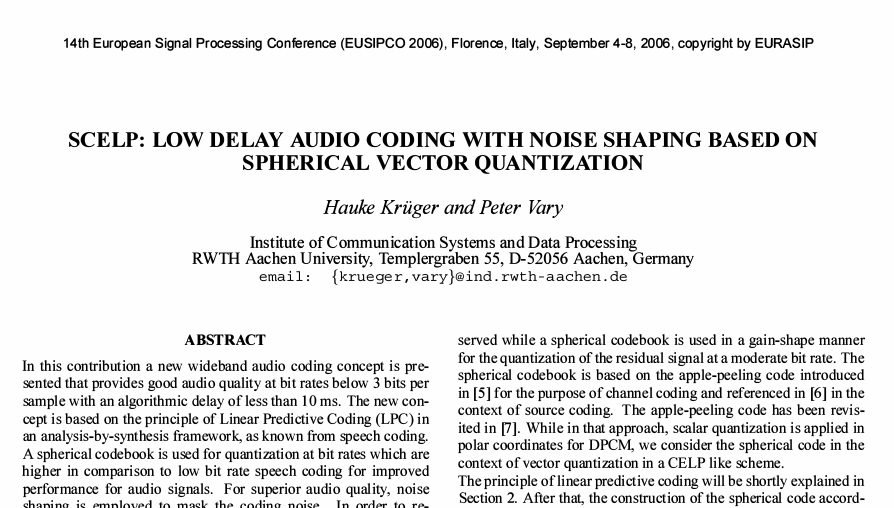
\includegraphics[width =0.5\linewidth]{./img/overview.png}
  \begin{itemize}
    \item Good audio quality at bit rates below 3 bits per sample
    \item Based in LPC with analysis-by-synthesis framework
    \item Spherical codebook for vectorial quatization
    \item Masked coding noise
    \item All-pole filter models spectral envelope of input signal
  \end{itemize}
  \begin{figure}
    \begin{minipage}{\textwidth}
            \footnotetext{[1] Proposal by Haunke Krüger and Peter Vary, both from the Aachen University, Germany. Published in 2006} \\
    \end{minipage}
\end{figure}
\end{frame}
%La propuesta de los autores consiste en un nuevo sistema para obtener calidad de audio a bit rates bajos (48 kbits/s). Para ello emplean un sistema basado en el Linear prediction coding usando analysis-by-synthesis (lazo cerrado) e integrando un codebook esferico para la cuatizacion(a explicar mas adelante). adicionalmente se emplea "noise shaping" para enmascarar el ruido de codificacion. El modelo empleado es el más habitual en el mundo de las comunicaciones y usa un filtro todo-polos para modelar la envolvente espectral de la entrada, y, en funcion de este filtro, se calcula el LP resiudal a traves del inverso del filtro anterior, el cual se cuantifica.

% SLIDE 2: _____________________________________________________________________
\begin{frame}{Adaptative Linear Prediction: Closed Loop Quantization }
\begin{itemize}
  \item Windowed segment of length $L_{lpc}$ to obtain coefficients LPC
  \item Coefficients must be sent together with the cuantized residual LP
  \item Vector quantization instead of scalar
\end{itemize}
\centering
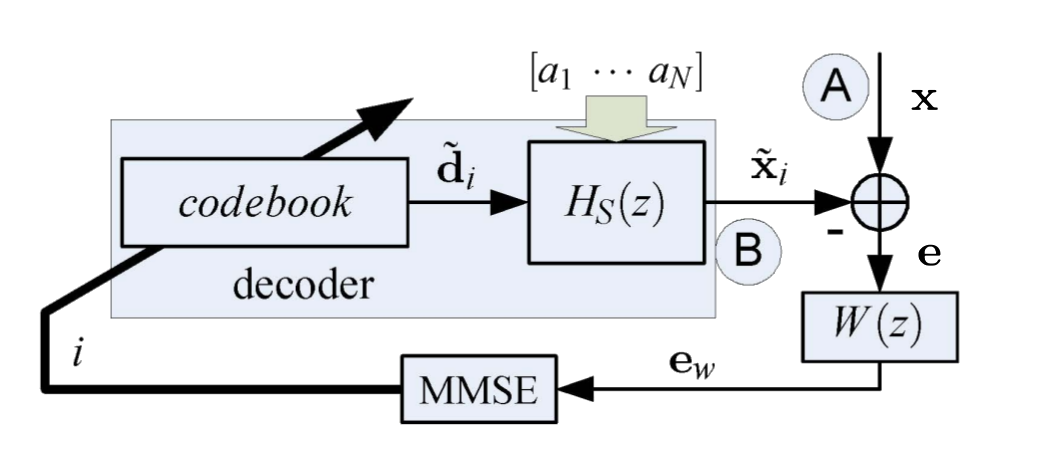
\includegraphics[width=0.8\linewidth]{./img/esquema_simple_r.png}
\end{frame}
% Al hacer prediccion lineal adapativa la señal de entrada se evalua en ventanas de longitud Llpc, a partir de dichas evalcuaciones se obitenen los coeficientes VARIANTES con los que se construye el filtro LP de ANALISIs, el cual nos da la señal residual LP. Dicha señal se cuantiza y transmite al decodificador. El filtro de SINTESIS (inverso del anterior) reconstruye la señal original (lo mejor que puede) a traves de dicho filtro en el decodificador. En el caso a tratar los coeficientes deben ser enviados junto con la señal residual cuantizada, esto supone un aumento no significante en el bit rate.

% Al usar cuantizacion vectorial (muchas nuestras de la señal LP residual se juntan en un vecttor de longitud Lv) se obtienen beneficios que no aparecen al usar la escalar. Para ello se emplea colsed loop en el lado del codificador, a través de esto se encuentra el vector cuantizado optimo  a usar como excitacion del LP residual. Explicar funcionamineto acompañado del esquema Figura 1: Analysis-by-synthesis for VQ


  % SLIDE : _____________________________________________________________________
  \begin{frame}{Optimized Excitation Search Modified}
    Complexity Reduction scheme:\\
      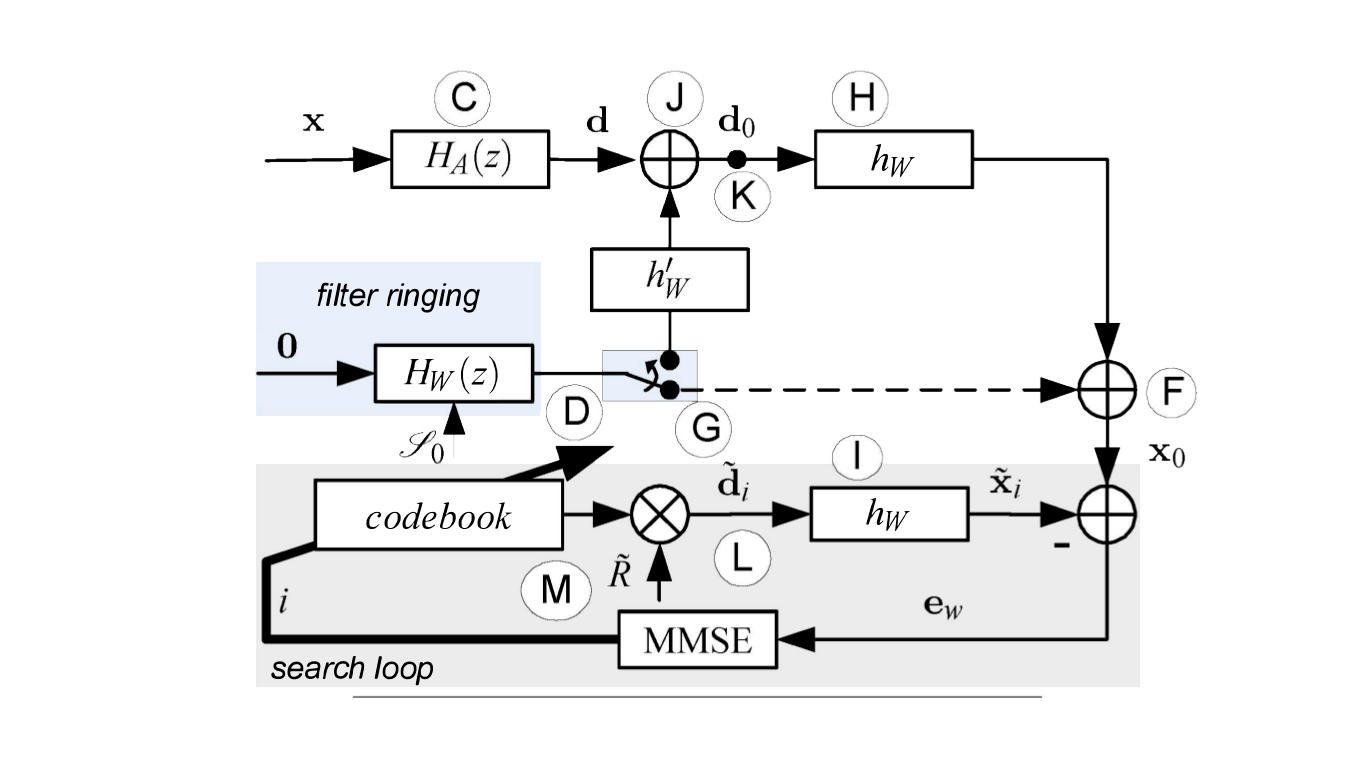
\includegraphics[width=\linewidth]{./img/closed_loop_scheme_complex.png}
              %Figure 3: modified analysis-by-synthesis

      %Dado que pueden haber muchos posibles vectores el sistema original se modifica para hacerlo más eficiente/facil de obtener, explciar el nuevo esquema. Se emplean dos tecnicas para reducir la complejidad: preselccion que reduce la complejidad y exclusiond e candidatos, que aunque añada ruido simplifica mucho la complejidad compuacional.

      \vspace{10pt}
      \begin{figure}
        \begin{minipage}{\textwidth}
                \footnotetext{$W(z) = H_{A}(z) * H_{s}(z) * W(z) = H_{A}(z)*H_{W}(z)$} \\
        \end{minipage}
    \end{figure}
  \end{frame}



  % SLIDE : _____________________________________________________________________
  \begin{frame}{Conclusion and Results}
    \begin{itemize}
      \item Sample rate 16kHz
      \item Lv = 11
      \item Outperforms G.722
      \item Encoder: 20-25 WMOPS
      \item Decoder: 1-2 WMOPS
      \item Bitrates below 48 Kbps
      %Comentar los numeros. WMOPS = weighted millions of operations per second. Conclusion: Usando un codebook esferico y procesos eficientes de seleccion se ha conseguido mejorar el CELP tradicional en 0.22MOS 3.83
    \end{itemize}
  \end{frame}

% SECTION 2:====================================================================

\begingroup
\setbeamercolor{section title}{fg=white}
\setbeamercolor{background canvas}{bg=mDarkTeal}
\section{Spherical Codebook}
\endgroup

% SLIDE : _____________________________________________________________________
\begin{frame}{Spherical Codebook}
  \begin{itemize}
    \item Codewords composed by:
    \begin{itemize}
      \item Gain (scalar)* \hspace{60pt}\footnotesize *We quantify it using a log quanifier
      \item Shape (vector)
    \end{itemize}
    \item Apple-peeling rule
    \end{itemize}
  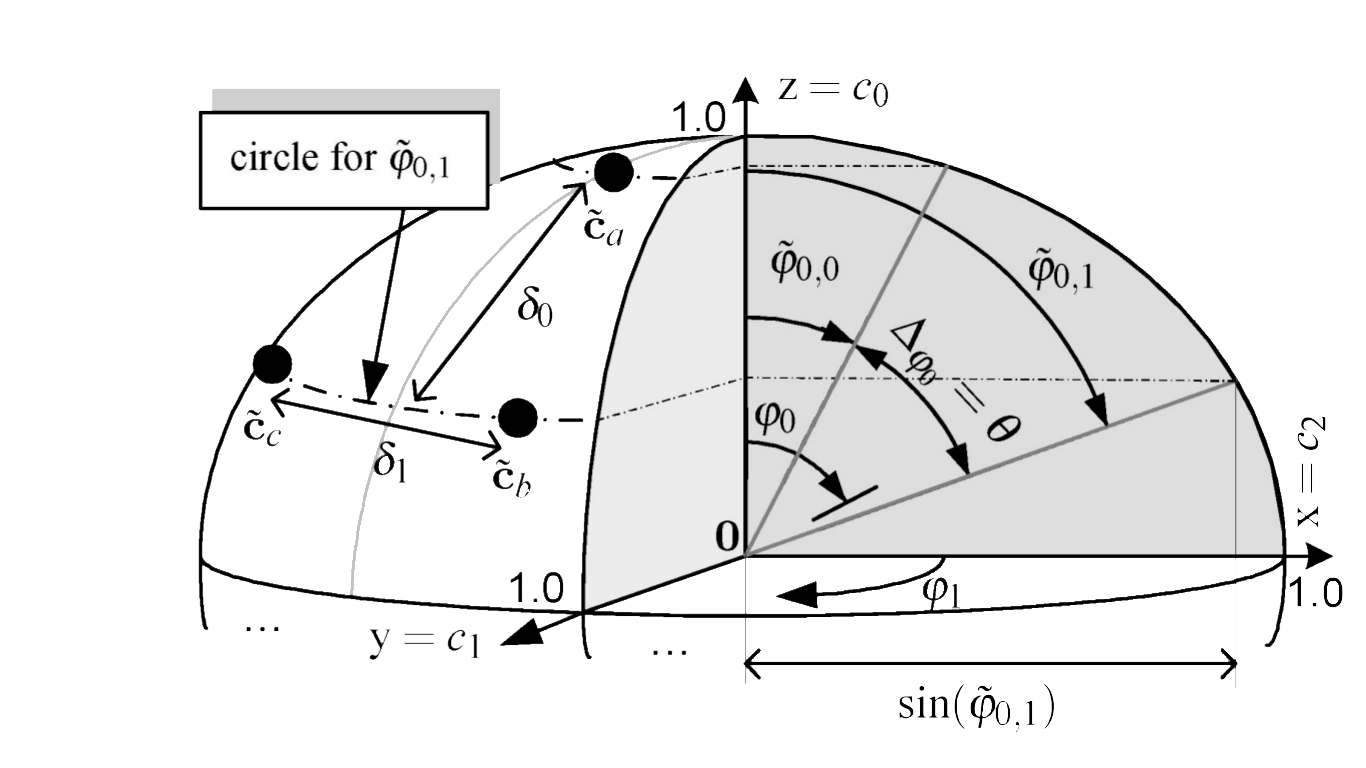
\includegraphics[width=0.9\linewidth]{./img/Centroides.png}
    % El codebook esferico tiene sus vectores compuestos por una ganancia (gain) que es un escalar y un vector llamado forma (shape). Los vectores están en el radio unidad de la esfera, y la ganancia es el radio cuantizado.
    % Se usa el metodo applepeeling para encontrar el codebook dentro del espacio Lv-dimensional. Conduicion de diseño : Llpc/Lv entero, para tener distribucion uniforme en el radio de la esfera
              %Figura 2: 3-dimensional sphere for apple-peeling code. explicarla bien.

\end{frame}

% SLIDE : _____________________________________________________________________
\begin{frame}{Spherical Codebook Construction: 3D model}
All layers expcept the last:
  \begin{itemize}
    \item Separation between layers:\\
    \begin{center}
      $\theta (N_{sp}) = \pi/N_{sp}$ where Nsp denotes the number of sublayers.
    \end{center}
    \item Angle for the next layer:\\
    \begin{center}
      $ \tilde{\phi}_{0,i_{0}} = (i_{0} + 1/2) \cdot \theta(N_{sp})$
    \end{center}

    % La esfera se divide en circulos separados pi/Nsp, de manera que la distancia entre circulos sera pi/Nsp, dichos circulos se encuentran en los angulos obtenidos por la expresion (4). Los centroides siguen la expresion (7), donde Nsp1 es el numero de itnervalos en cada circumferencia.
              % insertar ecuacion (4), (5), (6), (7)
  \end{itemize}
Last layer:
\begin{itemize}
  \item Number of centroids:\\
  \begin{equation*}
  N_{sp,1}(\tilde{\phi}_{0,i_{0}}) = \lfloor\frac{2\pi}{\theta(N_{sp})} \cdot sin(\tilde{\phi}_{0,i_{0}})\rfloor
  \end{equation*}
  \item Centroid angle:
  \begin{equation*}
    \tilde{\phi}_{1,i_{1}}(\tilde{\phi}_{0,i_{0}}) = (i_{1} + 1/2) \cdot \frac{2\pi}{N_{sp,1}(\tilde{\phi}_{0,i_{0}})}
  \end{equation*}

\end{itemize}
\end{frame}

% SLIDE : _____________________________________________________________________
\begin{frame}{Spherical Codebook: Cartesian Coordinates of centroids}
  \begin{itemize}
    \item Cartessian coordinates:\footnotemark\footnotetext{Font: Wikipedia}
    \begin{equation*}
      x_{1} = r \cdot cos(\phi_{1})
    \end{equation*}
    \begin{equation*}
      x_{2} = r \cdot sin(\phi_{1}) \cdot cos(\phi_{2})
    \end{equation*}
    \begin{equation*}
      x_{3} = r \cdot sin(\phi_{1}) \cdot sin(\phi_{2}) \cdot cos(\phi_{3})
    \end{equation*}
    \centering $\vdots$
    \begin{equation*}
      x_{n-1} = r \cdot sin(\phi_{1}) \cdot \dotsc \cdot sin(\phi_{n-2}) \cdot cos(\phi_{n-1})
    \end{equation*}
    \begin{equation*}
      x_{n} = r \cdot sin(\phi_{1}) \cdot \dotsc \cdot sin(\phi_{n-2})  \cdot sin(\phi_{n-1})
    \end{equation*}
              % insertar ecuacion (8)
    % Dado que la esfera no es necesariamente tridimensional pasar de coordenadas esfericas a cartesianas no es evidente. Proceso costoso computacionalmente reducido mediante uso de tablas con los valores. para todos las dimensiones menos la última: coseno del angulo * producto de los senos de los anteriores. Para el ultimo: producto de senos anteriores
  \end{itemize}
  \vspace{40pt}
  \begin{figure}
    \begin{minipage}{\textwidth}
            \footnotetext{[2] Font: Wikipedia: https://en.wikipedia.org/wiki/N-sphere} \\
    \end{minipage}
\end{figure}
\end{frame}

% SLIDE : _____________________________________________________________________
\begin{frame}{Spherical Codebook: N-Spherical Coordinates of Centroids}
  \begin{itemize}
    \item Spherical coordinates:\footnotemark
    \small
    \begin{equation*}
      r = \sqrt{x_{n}^2 + x_{n-1}^2 + \dotsc + x_{2}^2 + x_{1}^2}
    \end{equation*}
    \small
    \begin{equation*}
      \phi_{1} = arccot \frac{x_{1}}{\sqrt{x_{n}^2 + x_{n-1}^2 + \dotsc + x_{2}^2}} = arccos \frac{x_{1}}{\sqrt{x_{n}^2 + x_{n-1}^2 + \dotsc + x_{2}^2 + x_{1}^2}}
    \end{equation*}
    \small
    \begin{equation*}
      \phi_{2} = arccot \frac{x_{2}}{\sqrt{x_{n}^2 + x_{n-1}^2 + \dotsc + x_{3}^2}} = arccos \frac{x_{2}}{\sqrt{x_{n}^2 + x_{n-1}^2 + \dotsc + x_{2}^2}}
    \end{equation*}
    \centering $\vdots$
    \small
    \begin{equation*}
      \phi_{n-2} = arccot \frac{x_{n-2}}{\sqrt{x_{n}^2 + x_{n-1}^2}} = arccos \frac{x_{n-2}}{\sqrt{x_{n}^2 + x_{n-1}^2 + x_{n-2}^2}}
    \end{equation*}
    \small
    \begin{equation*}
      \phi_{n-1} = 2\cdot arccot\frac{x_{n-1} + \sqrt{x_{n}^2 + x_{n-1}^2}}{x_{n}}
    \end{equation*}
              % insertar ecuacion (8)
    % Dado que la esfera no es necesariamente tridimensional pasar de coordenadas esfericas a cartesianas no es evidente. Proceso costoso computacionalmente reducido mediante uso de tablas con los valores. para todos las dimensiones menos la última: coseno del angulo * producto de los senos de los anteriores. Para el ultimo: producto de senos anteriores
  \end{itemize}
  \begin{figure}
    \begin{minipage}{\textwidth}
            \footnotetext{[3] Font: Wikipedia: https://en.wikipedia.org/wiki/N-sphere} \\
    \end{minipage}
\end{figure}
\end{frame}

% SLIDE : _____________________________________________________________________
\begin{frame}{Preselection}
  \begin{itemize}
    \item Select neighbour centroids surrounding the unquantized signal
    \item  2 new layer candidates for each layer. Select the upper and lower circumferences for each $\phi_i$
    \item $2^{L_v -1}$ total neighbours which are the candidates
    % Se computa la distorsion de todos los vecinos y se utiliza aquel que introduzca menos distorsion. Se puede profundizar mas en este punto, pero al ser secundario y no saber la longitud de la totalidad lo dejare asi por ahora.
  \end{itemize}
  \centering
  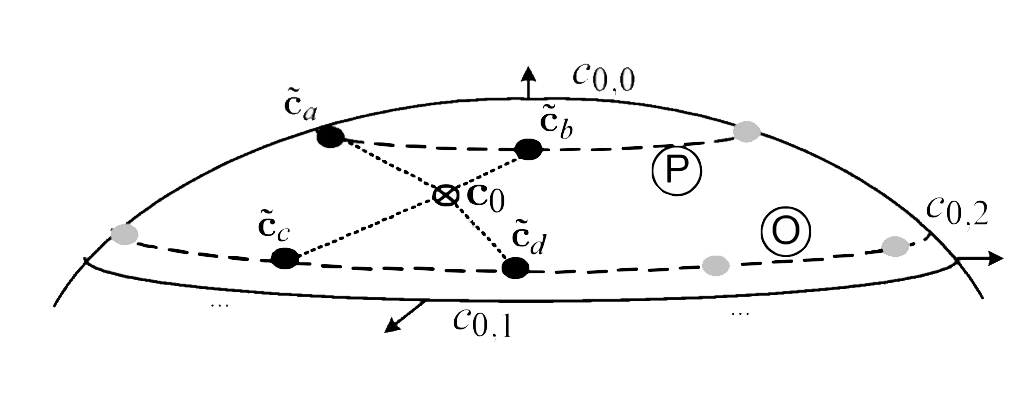
\includegraphics[width=\linewidth]{./img/optim_search_2.png}
\end{frame}

% SLIDE : _____________________________________________________________________
\begin{frame}{Candidate-exclusion}
\begin{center}
  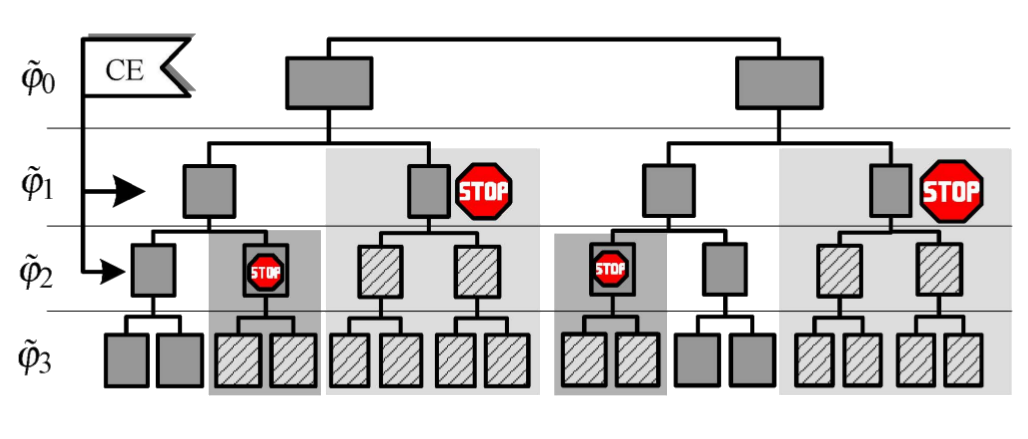
\includegraphics[width=\linewidth]{./img/arbre.png}
\end{center}
Minimize the partial distorsion\footnotemark:
  \begin{itemize}
    \item Reduce the computation complexity
    \item Loss in quatization SNR
    \end{itemize}

            %Figure 6: Candidate-exclusion (CE)
    % La exclusion de candidatos se hace en paralelo con la preseleccion. Una vez se han difinido los candidatos a traves de preseleccion se dividen los vecotres en subvectores, y ?????????????????????
    \begin{figure}
      \begin{minipage}{\textwidth}
              \footnotetext{[4] Partial Distortion: $D_{i} = \sum_{j=0}^{l_{0}}(x_{0,j} -\tilde{\textbf{x}}_{i,j}|_{[0 ... i_{0}]})^2$} \\
      \end{minipage}
    \end{figure}
\end{frame}

  % SECTION 3:====================================================================

  \begingroup
  \setbeamercolor{section title}{fg=white}
  \setbeamercolor{background canvas}{bg=mDarkTeal}
  \section{Our Implementation}
  \endgroup

  % SLIDE : _____________________________________________________________________
  \begin{frame}{Our Implementation: Open-Loop (Basic Idea)}
  Predict with the unquantized values
    \begin{itemize}
      \item Encoder:\\
        \begin{center}
        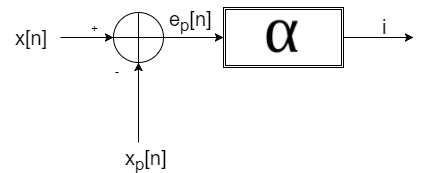
\includegraphics[width=0.6\linewidth]{./img/Esquema_1.png}
        \end{center}
      \item Decoder:\\
      \begin{center}
        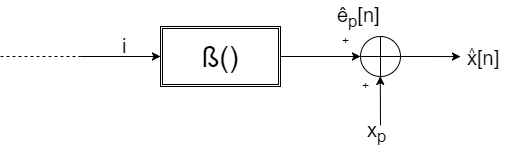
\includegraphics[width=0.7\linewidth]{./img/Esquema_2.png}
      \end{center}
    \end{itemize}
  \end{frame}
  % SLIDE : _____________________________________________________________________
  \begin{frame}{Our Implementation: Open-Loop (Advanced Scheme)}
  Use the quantized values in the predictor
  \begin{itemize}
    \item Encoder:\\
      \begin{center}
      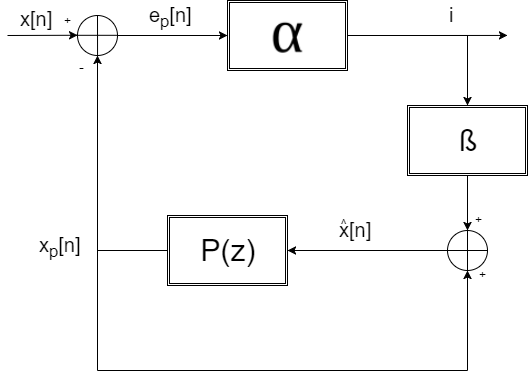
\includegraphics[width=0.45\linewidth]{./img/Esquema_3.png}
      \end{center}
    \item Decoder:\\
    \begin{center}
    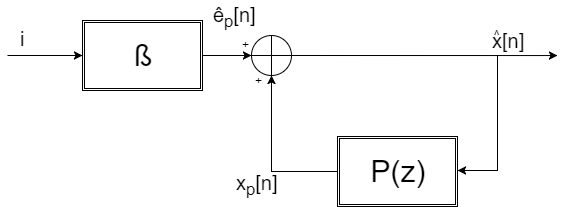
\includegraphics[width=0.55\linewidth]{./img/Esquema_4.png}
    \end{center}
  \end{itemize}
  \end{frame}

  % SECTION 4:====================================================================

  \begingroup
  \setbeamercolor{section title}{fg=white}
  \setbeamercolor{background canvas}{bg=mDarkTeal}
  \section{Our Simulations $\&$ Results}
  \endgroup
  % SLIDE :

  \begin{frame}{Route-Map}
  \begin{itemize}
    \item Test the codebook
    \item Test the open-loop scheme (basic)
    \item Compare with uniform quanitfier
  \end{itemize}

  Metrics:


  \centering
    $SNR = 10log(\frac{P_{x_p}}{P_e_q})$ \\
    $P_e_q = \frac{1}{N}\sum e_q^2$\\
    $P_x_p = \frac{1}{N}\sum x_p^2$\\
    Prediction error: $e_q = x_p - \hat{x_p} $\\
    Original signal: $x_p$\\
    Quantified signal: $\hat{x_p}$\\

  \end{frame}

  %_____________________________________________________________________
  \begin{frame}{Spherical Codebook Testing: ($l_v$, $N_{sp}$, $M_r$)=(3,20,6)}
    \begin{center}
    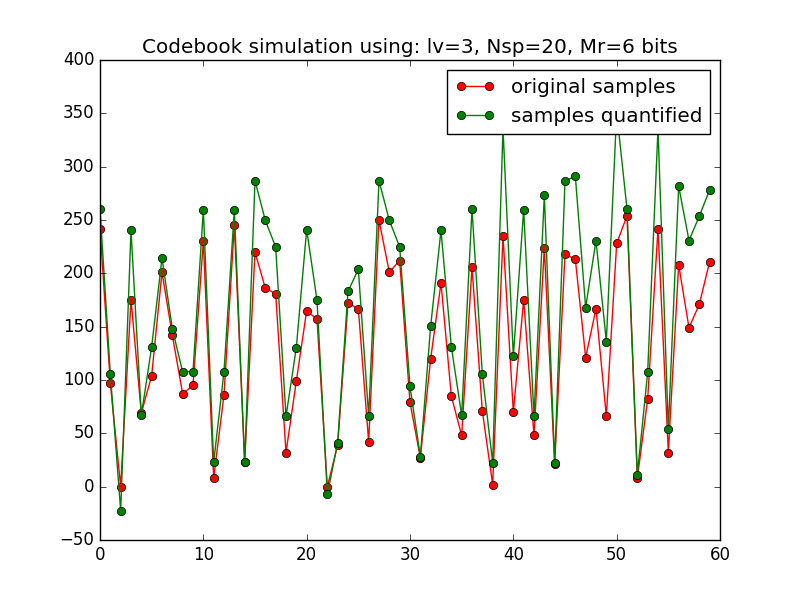
\includegraphics[width=0.8\linewidth]{./img/cb_3_20_6_r.png}\\
    \end{center}
    Number of centroids: 429 $\rightarrow$ 9 bits\\
    $SNR = 8.68 dB$\\
    Reduction: $24/15$ ($38\%$)
  \end{frame}

  % SLIDE : _____________________________________________________________________
  \begin{frame}{Spherical Codebook Testing: ($l_v$, $N_{sp}$, $M_r$)=(10,3,6)}
    \begin{center}
    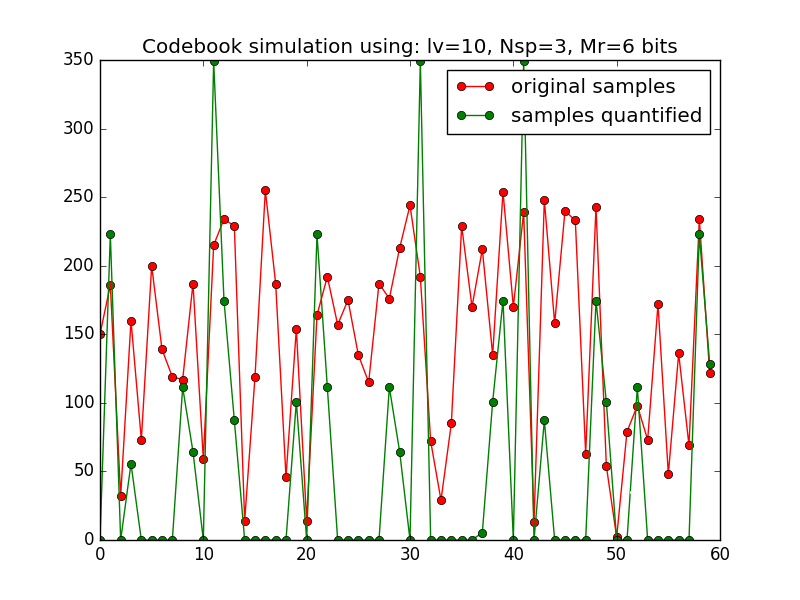
\includegraphics[width=0.8\linewidth]{./img/cb_10_3_6_r.png}\\
    \end{center}
    Number of centroids: 26244 $\rightarrow$ 15 bits\\
    $SNR = 1.73 dB$\\
    Reduction: $80/21$ ($73.7\%$)
  \end{frame}

  % SLIDE : _____________________________________________________________________
  \begin{frame}{Spherical Codebook Testing: ($l_v$, $N_{sp}$, $M_r$)=(5,10,6)}
    \begin{center}
    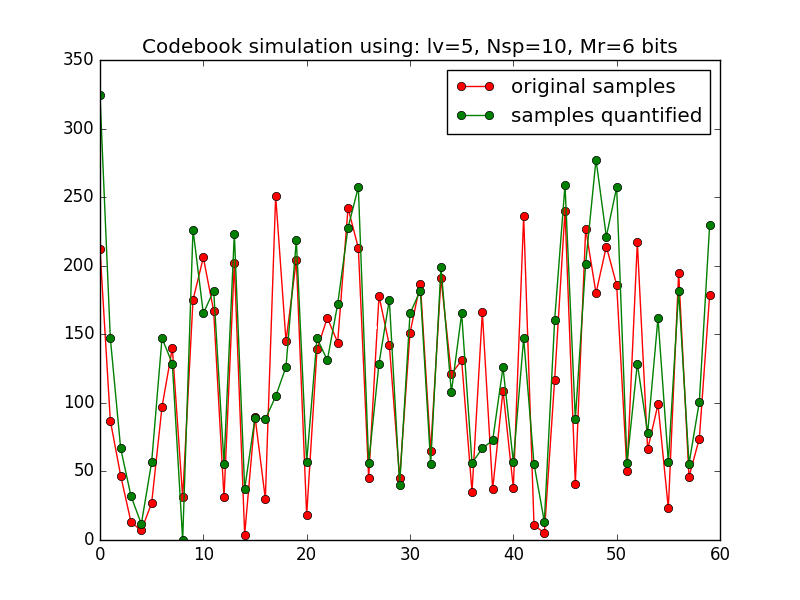
\includegraphics[width=0.8\linewidth]{./img/cb_5_10_6_r.png}\\
    \end{center}
    Number of centroids: 12400 $\rightarrow$ 14 bits\\
    $SNR = 7.85 dB$\\
    Reduction: $40/20$ ($50\%$)
  \end{frame}


  % SLIDE : _____________________________________________________________________
  \begin{frame}{General Prediction: Using the Basic Scheme}
  Using the predictor based on the unquanitzed values:
    \begin{center}
    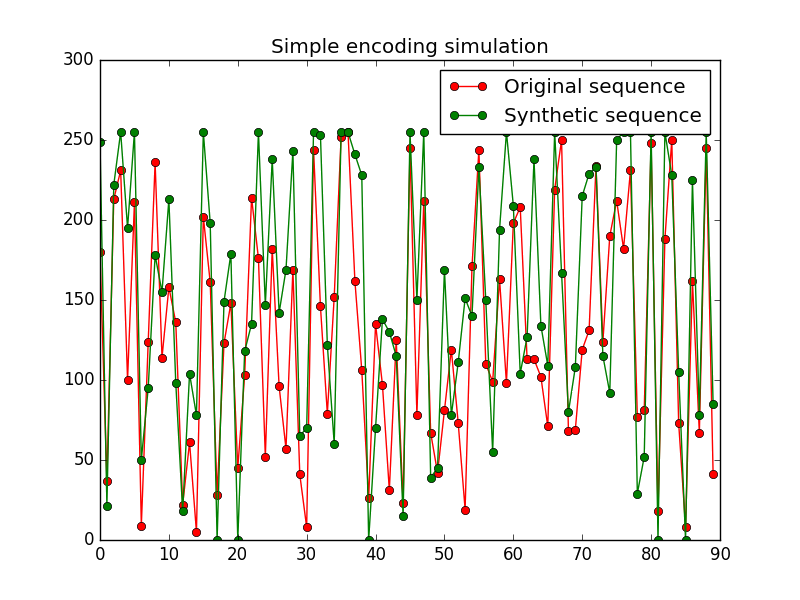
\includegraphics[width=0.7\linewidth]{./img/general_prediction_bo.png}\\
    \end{center}
    Codebook definiton: ($l_v$, $N_{sp}$, $M_r$)=(5,10,6) $\rightarrow$ 20 bits/ 5 samples\\
    $SNR = 8.05 dB$\\
    Reduction: $40/20$ ($50\%$)
  \end{frame}

  % SLIDE : _____________________________________________________________________
  \begin{frame}{Error Prediction Test}
    \begin{center}
    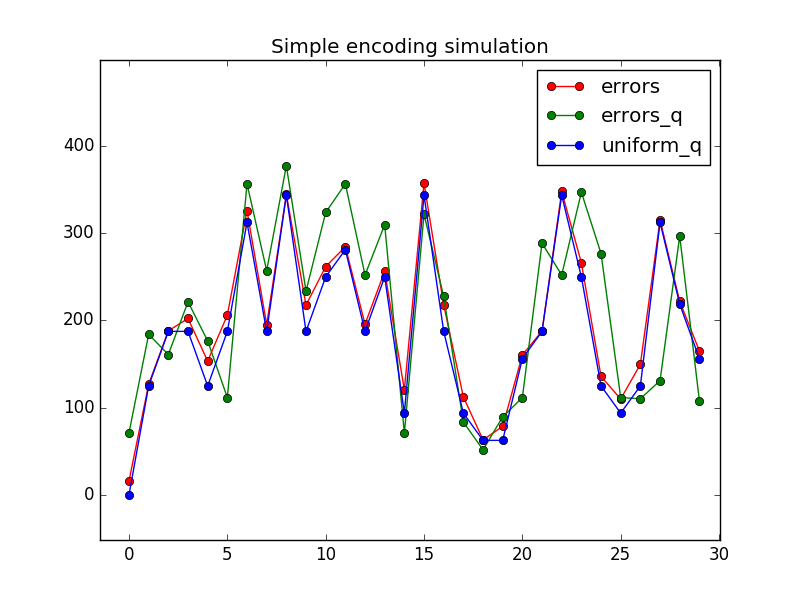
\includegraphics[width=0.75\linewidth]{./img/Bona_comparativa.png}\\
    \end{center}
    Codebook definiton: ($l_v$, $N_{sp}$, $M_r$)=(5,10,6) $\rightarrow$ 20 bits / 5 samples\\
    Uniform quantifier: 4 bits/sample\\
    $SNR_{spherical} = 10.8\ dB$\\
    $SNR_{uniform} = 22.4\ dB$\\
  \end{frame}

  % SLIDE : _____________________________________________________________________
  \begin{frame}{Error Prediction Test}
    \begin{center}
    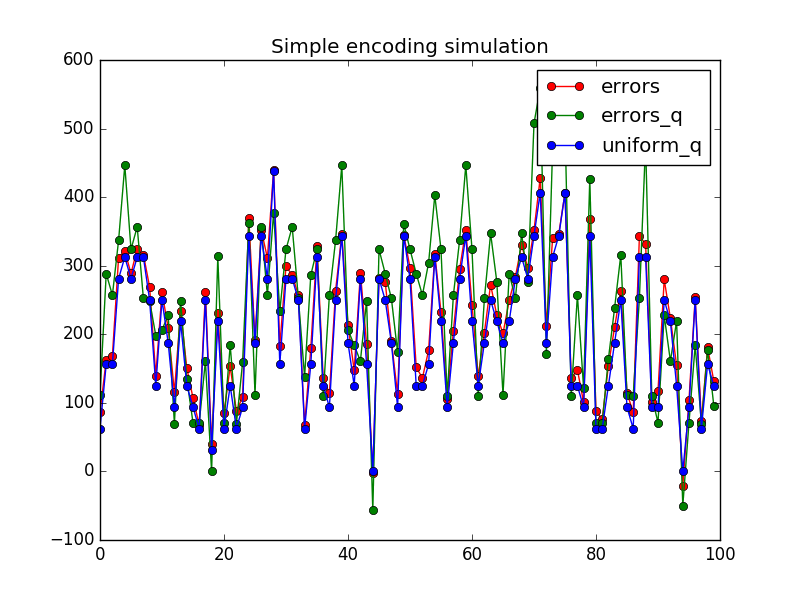
\includegraphics[width=0.75\linewidth]{./img/Bona_comparativa_moltes_mostres.png}\\
    \end{center}
    Codebook definiton: ($l_v$, $N_{sp}$, $M_r$)= $\rightarrow$ 20 bits / 5 samples\\
    Uniform quantifier: 4 bits/sample\\
    $SNR_{spherical} = 10.8\ dB$\\
    $SNR_{uniform} = 22.4\ dB$\\
  \end{frame}


  % SECTION 5:====================================================================

  \begingroup
  \setbeamercolor{section title}{fg=white}
  \setbeamercolor{background canvas}{bg=mDarkTeal}
  \section{Conclusions}
  \endgroup

  % SLIDE : _____________________________________________________________________
  \begin{frame}{Conclusions}
    \begin{itemize}
      \item Low bitrate coding acomplish
      \item Too complex model scheme
      \item Open-loop configuration can behave unexpectedly
      \item Big dimentional CB $\rightarrow$ great time-consuming impact
      \item Further improves are needed
    \end{itemize}
  \end{frame}



% ENDING: ======================================================================


\maketitle

\end{document}
